\chapter{Background}\label{background}

\minitoc

This chapter presents an overview of the core concepts critical to the foundation of this project, centering specifically on data visualization within the context of healthcare research. Additionally, it outlines the crucial technical tenets that form the backbone of software development, important for understanding the subsequent material.

\section{Data Visualization}\label{data-visualization}

Data visualization serves various aims, such as exploration,
interpretation, and communication of data, by harnessing human visual
perceptual abilities
\cite{5}. The field is
inherently complex, integrating elements of creativity, technology, and
social knowledge to achieve its goals. This complexity echoes the
diverse requirements and challenges seen in healthcare research, where
visualization tools must be both scientifically rigorous and accessible
for diverse stakeholders.

\subsection{Historical Development and
Evolution}\label{historical-development-and-evolution}

Historically, visualization techniques have been distributed mainly as
stand-alone applications or specialized libraries. This practice is
particularly prevalent for niche or highly specialized visualization
methods. However, over time, there has been a shift towards
generalization and abstraction. Developers have distilled components
from these specialized solutions to create general-purpose frameworks.
These frameworks assist in crafting custom visual representations,
providing a more flexible toolset for different applications, including
healthcare research \cite{5}.

The evolution of visualization tools and techniques in healthcare is a testament to the field's ongoing quest to enhance the understanding and communication of complex data. The story begins with an iconic figure in healthcare history: Florence Nightingale, whose innovative work during the Crimean War laid the groundwork for modern data visualization. Nightingale's use of polar area diagrams, or coxcombs, revolutionized the way data was presented to the British parliament and played a pivotal role in reforming military and public health practices. Figure \ref{fig:coxcomb} illustrates Nightingale's visualization of mortality causes among soldiers, distinguishing deaths due to preventable diseases, wounds, and other causes through a vivid color scheme. This early example underscores the power of visualization to not only convey statistics but also to advocate for change \cite{soa7}.

\begin{figure}[ht]
  \centering
  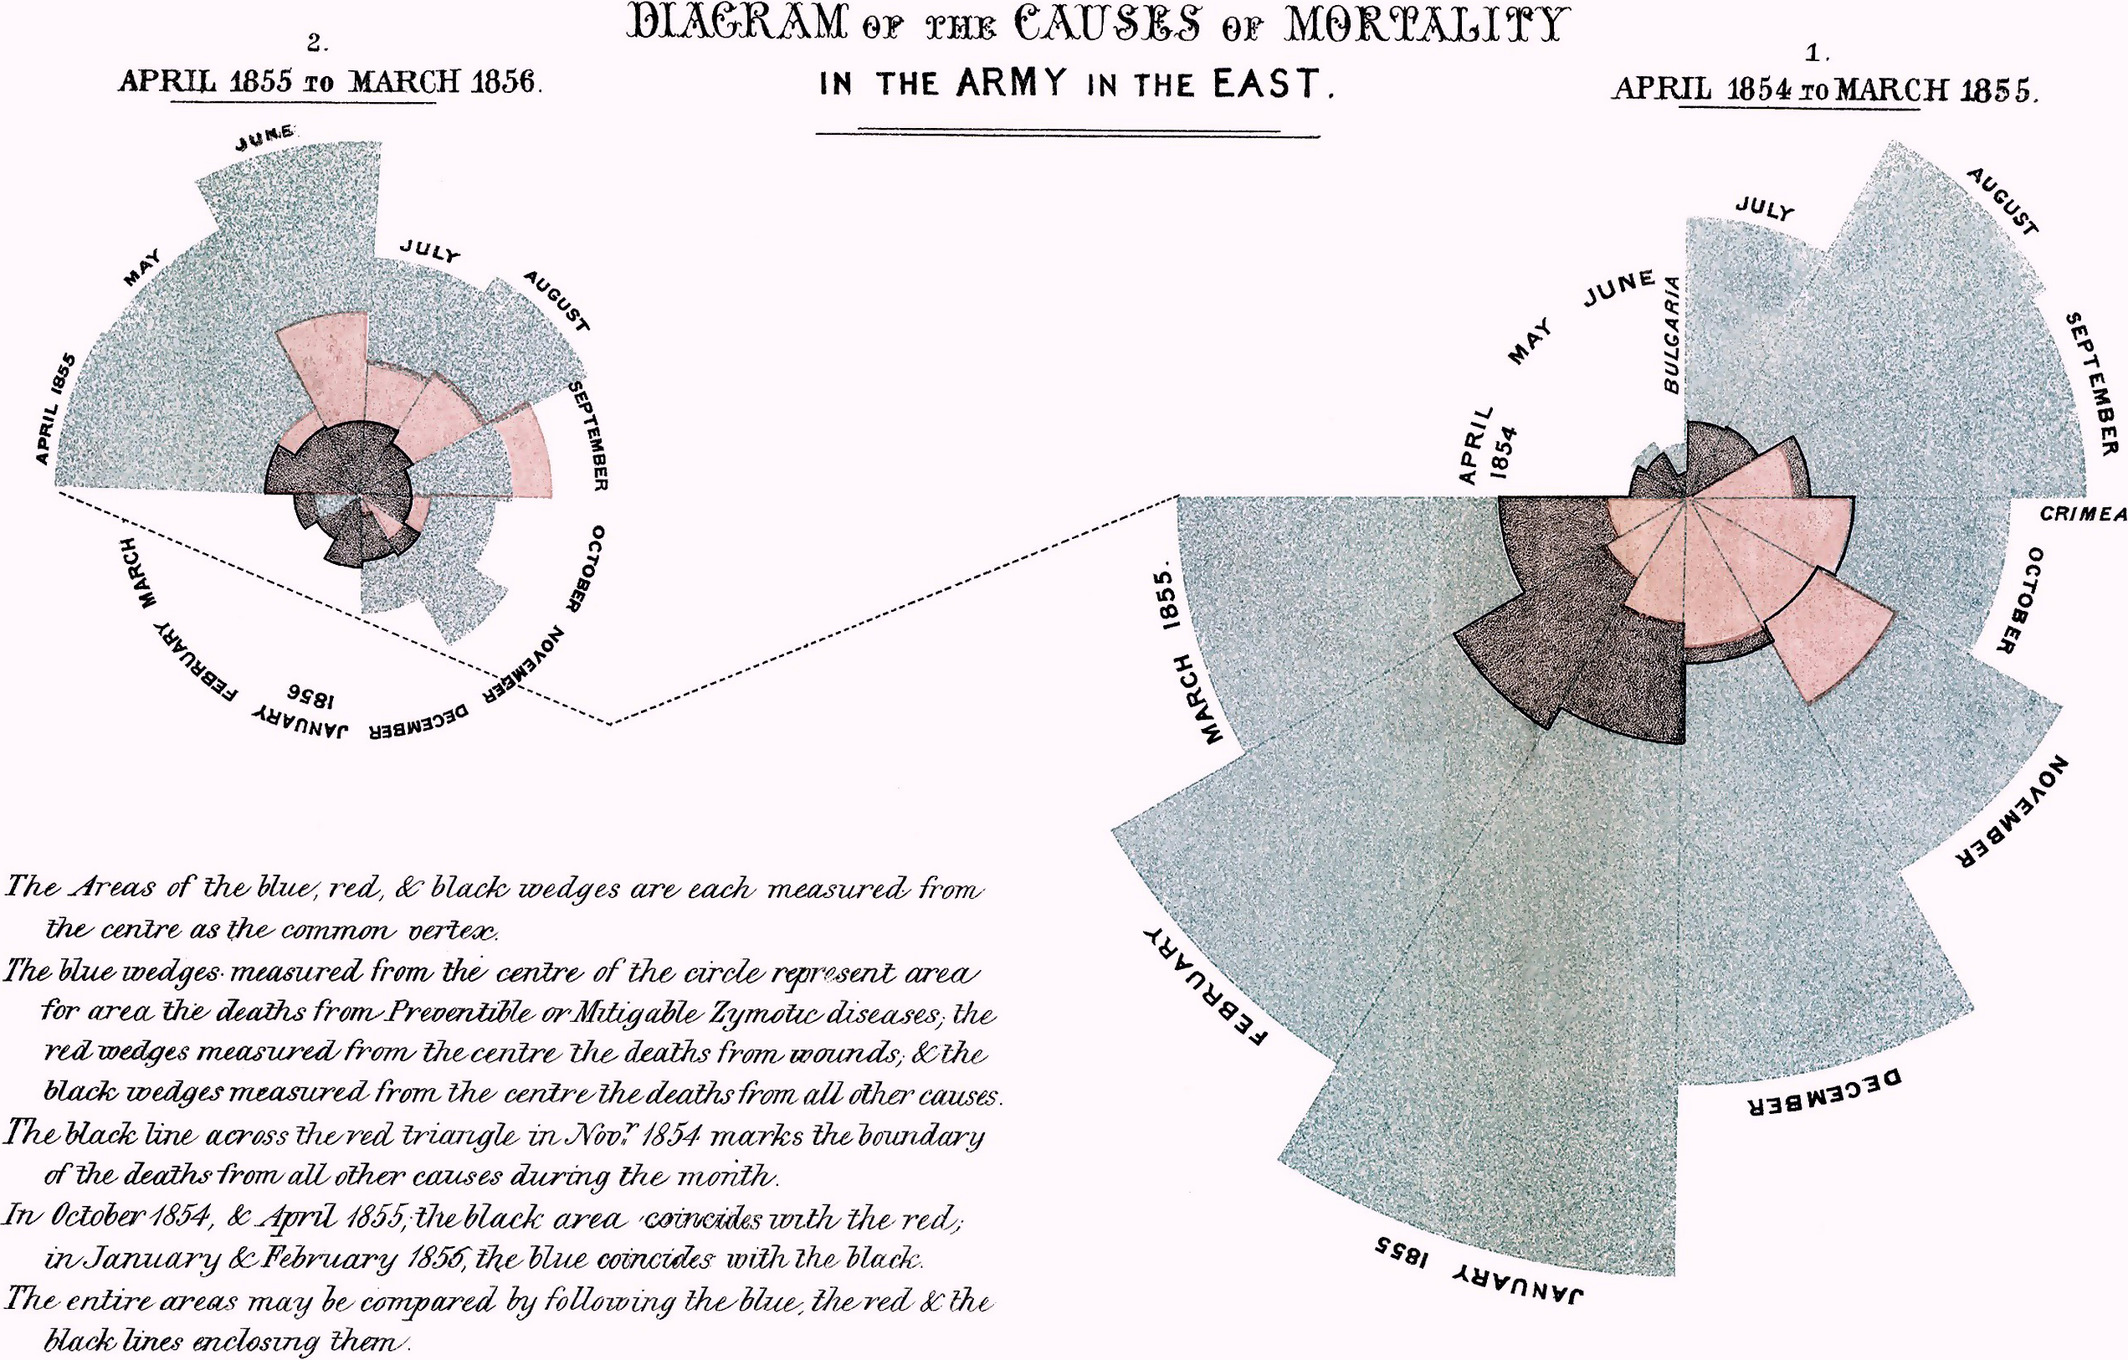
\includegraphics[width=\textwidth]{media/fig20.jpeg}
  \caption{Nightingale's coxcomb diagram on causes of mortality in the British army. Reproduced from O'connor \textit{et al} (2017)\cite{soa7}.}
  \label{fig:vsc}
\end{figure}

Today's healthcare industry, driven by data and evidence-based practice, continues to rely on the effective presentation of information. The plethora of digital health data from electronic medical records, telehealth systems, and wearable devices necessitates innovative visualization approaches to inform decisions and policies.

The science of data visualization has since matured, offering sophisticated representations of genomic, clinical, and personal health data to facilitate quick assimilation of information by diverse stakeholders.

\subsection{Design Choices}\label{design-choices}

To appreciate the role of visualizations in today\textquotesingle s
research landscape, it\textquotesingle s critical to analyze their
evolution and the importance of their design. Over the last three
centuries, charts, graphs, and equivalent visual representations have
become primary mediums for quantitative communication
\cite{6}.

Despite their increasing use, visualization designers have to navigate
through multiple decisions. This includes the choice of visual encoding
and styling, which significantly influences the aesthetics and
perception of a graphic
\cite{7}. Unfortunately,
though principles of effective visualization design have seen
significant development, many contemporary charts exhibit substandard
design choices that interfere with comprehension and aesthetic appeal.
However, incorporating automated design methods based on established
visual design principles can improve the effectiveness and consistency
of visualizations, particularly for analysts working with their own data
\cite{8}.

\subsection{Graphics Grammars}\label{graphics-grammars}

One foundational line of research in this field has been the systematic
study of structural theories of graphics, which is thought to have been
introduced by Bertin \cite{9}. In this research statistical graphics were deconstructed into their basic elements such as rectangles, lines or points. This in turn led to the development of
graphical languages. These languages enable a wide array of graphical
representations through the combination of simple geometric primitives
and transformations \cite{5}.

In the field of data visualization, the term "Graphics Grammars" refers
to a methodological approach to the creation and manipulation of visual
displays using structured, syntax-like rules and principles. Derived
from language theory, grammar here doesn\textquotesingle t pertain to
linguistic rules; instead, it represents a system of structures and
transformations that directs the visual representation of data. Graphics
grammars enable a more systematic and succinct specification of
graphics, which can be a real advantage in large-scale, complex data
visualization projects.

Low-level grammars such as Protovis \cite{10}, D3 \cite{11}, and Vega \cite{12} are often beneficial for explanatory data visualization or creating customized analysis tools due to their primitives offering fine-grained control.
For exploratory visualization, however, higher-level grammars like
ggplot2 \cite{13}, are
usually preferred for their conciseness over expressiveness. Another
example of a higher-level grammar is Vega-Lite, that provides a more
concise interface than the lower-level Vega language, making systematic
enumeration and ranking of data transformations and visual encodings
more manageable \cite{14}. A
summary of various graphics grammars and their characteristics is
provided in Table \ref{tab:graph_grammar}.

% Please add the following required packages to your document preamble:
% \usepackage{booktabs}
\begin{table}[ht]
  \caption{Summary of Graphics Grammar Languages}
  \label{tab:graph_grammar}
  \begin{tabular}{@{}llll@{}}
  \toprule
  \textbf{Language}    & \textbf{Level} & \textbf{Implementation}                                          & \textbf{Notable Features}                                                                                                                                                                                                                                         \\ \midrule
  \textbf{Protovis}    & Low            & JavaScript                                                       & \begin{tabular}[c]{@{}l@{}}No longer under active development, the responsible \\ team is now maintaining D3.js (see below).\end{tabular}                                                                                                                         \\ \midrule
  \textbf{D3.js}       & Low            & JavaScript                                                       & \begin{tabular}[c]{@{}l@{}}Capable of generating interactive data visualizations, \\ including transitions and tooltips, using web \\ technologies. Typical use cases include the creation \\ of custom visualizations.\end{tabular}                              \\ \midrule
  \textbf{Vega}        & Low            & \begin{tabular}[c]{@{}l@{}}JavaScript/\\ TypeScript\end{tabular} & \begin{tabular}[c]{@{}l@{}}The visualization is defined in a JSON format. \\ Typical use cases include the creation of explanatory \\ figures, with high degree of customization.\end{tabular}                                                                    \\ \midrule
  \textbf{ggplot2}     & High           & R                                                                & \begin{tabular}[c]{@{}l@{}}Part of the tidyverse, a collection of R packages \\ designed for data science. Based on the concept of \\ the "Grammar of Graphics," initially proposed by \\ Leland Wilkinson. Widely-used in the academic \\ community\end{tabular} \\ \midrule
  \textbf{Vega-Lite}   & High           & TypeScript                                                       & \begin{tabular}[c]{@{}l@{}}Enables the use of higher-level grammar, defined \\ using JSON format,  that is compiled to Vega \\ specifications. Typical use cases include the \\ creation of quick exploratory data visualizations.\end{tabular}                   \\ \midrule
  \textbf{Vega-Altair} & High           & Python                                                           & \begin{tabular}[c]{@{}l@{}}Leverages the Vega-Lite JSON specification and \\ creates a declarative Python API for the creation \\ of visualizations.\end{tabular}                                                                                                 \\ \midrule
  \textbf{Matplotlib}  & Low            & Python                                                           & \begin{tabular}[c]{@{}l@{}}One of the most popular python libraries for data \\ visualization. Notable for extensive customization \\ and ability to generate 2D and 3D Plots.\end{tabular}                                                                       \\ \bottomrule
  \end{tabular}
  \end{table}

\subsubsection{Visualizations in the Study
Lifecycle}\label{visualizations-in-the-study-lifecycle}

Visualizations have a vital role throughout the lifecycle of any
research study. They provide key insights during crucial stages such as
\cite{15}:

\begin{itemize}
  \item \textbf{Protocol development}: Visualizations aid in analyzing design
  and data issues clearly and objectively, ensuring study accuracy.
  \item \textbf{Diagnostics}: They assist in verifying if all prerequisites
  for the study have been met, including the requirements set by the
  chosen statistical methods.
  \item\textbf{Results}: Visual data representations help to interpret
  research outcomes enhancing communication and understanding.
\end{itemize}


The role of visualizations throughout various stages of a research study
underscores the necessity for specialized tools capable of adapting to
the complex demands of healthcare research. VV aims to address some of
these needs by automating the visualization creation process.

\section{Technical Foundations and Development
Paradigms}\label{technical-foundations-and-development-paradigms}

This section will outline some key principles that have guided the
architecture and functionalities of robust and scalable software
systems.

\subsection{Modularity}\label{modularity}

The idea of modularity has a long history in the field of software
development. As early as 1970, Gouthier and Pont outlined the critical
elements of system modularity in their textbook on system program
design, stating that well-defined project segmentation ensures each task
forms a distinct program module. This clarity in definition streamlines
the implementation, testing, and even maintenance phases of development,
making it easier to trace errors and deficiencies to specific system
modules \cite{16}.

Parnas\textquotesingle{} seminal paper in 1972 further evolved the
philosophy by introducing the concept of "information hiding" in modular
programming, laying the groundwork for what later came to be termed as
high cohesion and loose coupling
\cite{17}\cite{18}. This
evolution was particularly important for large codebases, offering a
framework that allows modules to be written, reassembled, and replaced
without needing to reassemble the entire system
\cite{17}.

Beyond the code itself, the systematic reuse of software modules offers
a series of additional benefits. This approach not only improves
software dependability but also reduces process risks and accelerates
development cycles
\cite{19}. These advantages
are particularly important in healthcare settings where the need for
reliable and timely solutions is ever-present.

The importance of conceptual integrity in software design
shouldn\textquotesingle t be underestimated either. In his 1975 book,
"The Mythical Man-Month: Essays on Software Engineering," Brooks
advocated for the architecture of a system to be designed by a single
mind or a small, cohesive team to ensure a consistent and
well-thought-out framework
\cite{20}.

Overall, the benefits of a modular design approach are far-reaching.
They contribute collectively to enhancing productivity and software
quality, significantly reducing both time-to-market and development
costs \cite{19}. In fields
like healthcare, the positive impacts of adopting a modular design
philosophy can be particularly impactful.

\subsection{Object-Oriented Programming
(OOP)}\label{object-oriented-programming-oop}

OOP has been a common paradigm for solving complex tasks through
interactions between objects. It allows for greater flexibility, better
quality coding techniques, and enhanced productivity
\cite{21}\cite{22}. With the
project's complexity and the need for a clear, modular structure, OOP
becomes an ideal choice. OOP languages like C++, Python, and Java have
dominated software development, making them crucial for both current and
future applications
\cite{23}\cite{24}.

While OOP offers many advantages, it is not without limitations.
Complexity control remains a challenge, especially when these codes are
updated to cover future requirements
\cite{21}\cite{25}. This
complexity often results from the very features that make OOP powerful:
polymorphism, inheritance, and encapsulation.

To manage this complexity, several design principles and patterns have
been introduced. The Gang of Four\textquotesingle s design patterns
provide robust frameworks for addressing recurrent design issues,
focusing on creational, structural, and behavioral patterns. These
patterns help in making OOP code more manageable, reusable, and
maintainable \cite{26}.
Furthermore, the Unified Modeling Language (UML) has been instrumental
in providing a general-purpose language for visualizing, specifying,
constructing, and documenting the artifacts of software systems. It aids
both developers and business stakeholders throughout the software
modeling process \cite{27}.
To enhance code quality and manage complexity, principles such as the
SOLID principles have been proposed, promoting design that is easy to
manage and scale
\cite{24}\cite{28}.

\subsection{Test-Driven Development
(TDD)}\label{test-driven-development-tdd}

The field of software development offers a variety of methodologies
aimed at optimizing code quality, increasing efficiency, and promoting
teamwork. Among these, Test-Driven Development (TDD) is notable for its
iterative approach that integrates programming, unit testing, and code
refactoring.

TDD promotes the writing of automated tests before the actual production
code is developed. This proactive approach has been shown to lead to
projects of higher quality that are completed in a shorter period
compared to traditional methods. One added benefit is the generation of
a regression-test suite as a natural outcome, minimizing the need for
manual testing while allowing for earlier error detection and quicker
remediation. Traditional software development often involves
considerable time and resources dedicated to debugging in later stages.
TDD, however, facilitates testing early in the design cycle,
significantly reducing the time and financial resources spent on
debugging \cite{29}. This can
mitigate some of the complexity control issues that are often seen in
OOP \cite{23}\cite{25}.

In the TDD methodology, refactoring plays a crucial role, enabling
ongoing improvements in the internal structure of the code while
preserving its external behavior. This is beneficial for code
maintainability and long-term project viability
\cite{30}. TDD encourages
modular code, which aligns with the OOP principle of high cohesion and
loose coupling introduced by Parnas
\cite{17}\cite{24}. This
makes it easier to maintain and extend the system, thus enhancing
productivity, which represents a key advantage of OOP.

TDD is versatile, compatible with a range of software development
paradigms such as Agile, Scrum, XP, and Lean. This adaptability offers
flexibility in project management approaches
\cite{31}.

\subsection{Python Programming
Language}\label{python-programming-language}

The landscape of programming languages is ever-changing, but Python has
consistently shown remarkable growth both in the educational sector and
the industry at large. Python\textquotesingle s straightforward syntax
and robust set of tools position it as an ideal language for educational
settings, particularly for those new to programming.
It\textquotesingle s the go-to introductory language at many top-tier
universities, facilitating a seamless transition from basic mathematical
reasoning to intricate coding tasks. When compared to languages like
Java and C++, Python offers easier code writing, thanks in part to its
clean syntax, which is especially beneficial for educational
environments \cite{32}.

According to RedMonk\textquotesingle s programming language rankings, as
depicted in Figure \ref{fig:prog_lang}, Python has ascended to the second position as of
2023, right behind JavaScript. This ranking reflects a combination of
GitHub repositories and Stack Overflow discussions, providing insights
into both code usage and community discussion. The methodology
doesn\textquotesingle t claim to offer a statistically valid
representation of current usage but rather aims to provide insights into
potential future adoption trends
\cite{33}.

A comprehensive survey by Stack Overflow, which gathered responses from
89,184 software developers across 185 countries, revealed that Python is
the second most popular programming language in 2023, trailing only
behind JavaScript (64\% to 49\%, respectively). Python emerged as the
most favored language among non-professional coders. In the educational
sector, Python\textquotesingle s impact was also pronounced: 57\% of
student developers reported using Python, a figure that closely trails
JavaScript\textquotesingle s 61\%, further underscoring
Python\textquotesingle s growing significance in educational settings.
Note that in our the interpretation of the survey data categories such
as HTML/CSS and SQL were deliberately excluded from this analysis due to
their unique and complementary roles in software development
\cite{34}.

\begin{figure}[ht]
  \centering
  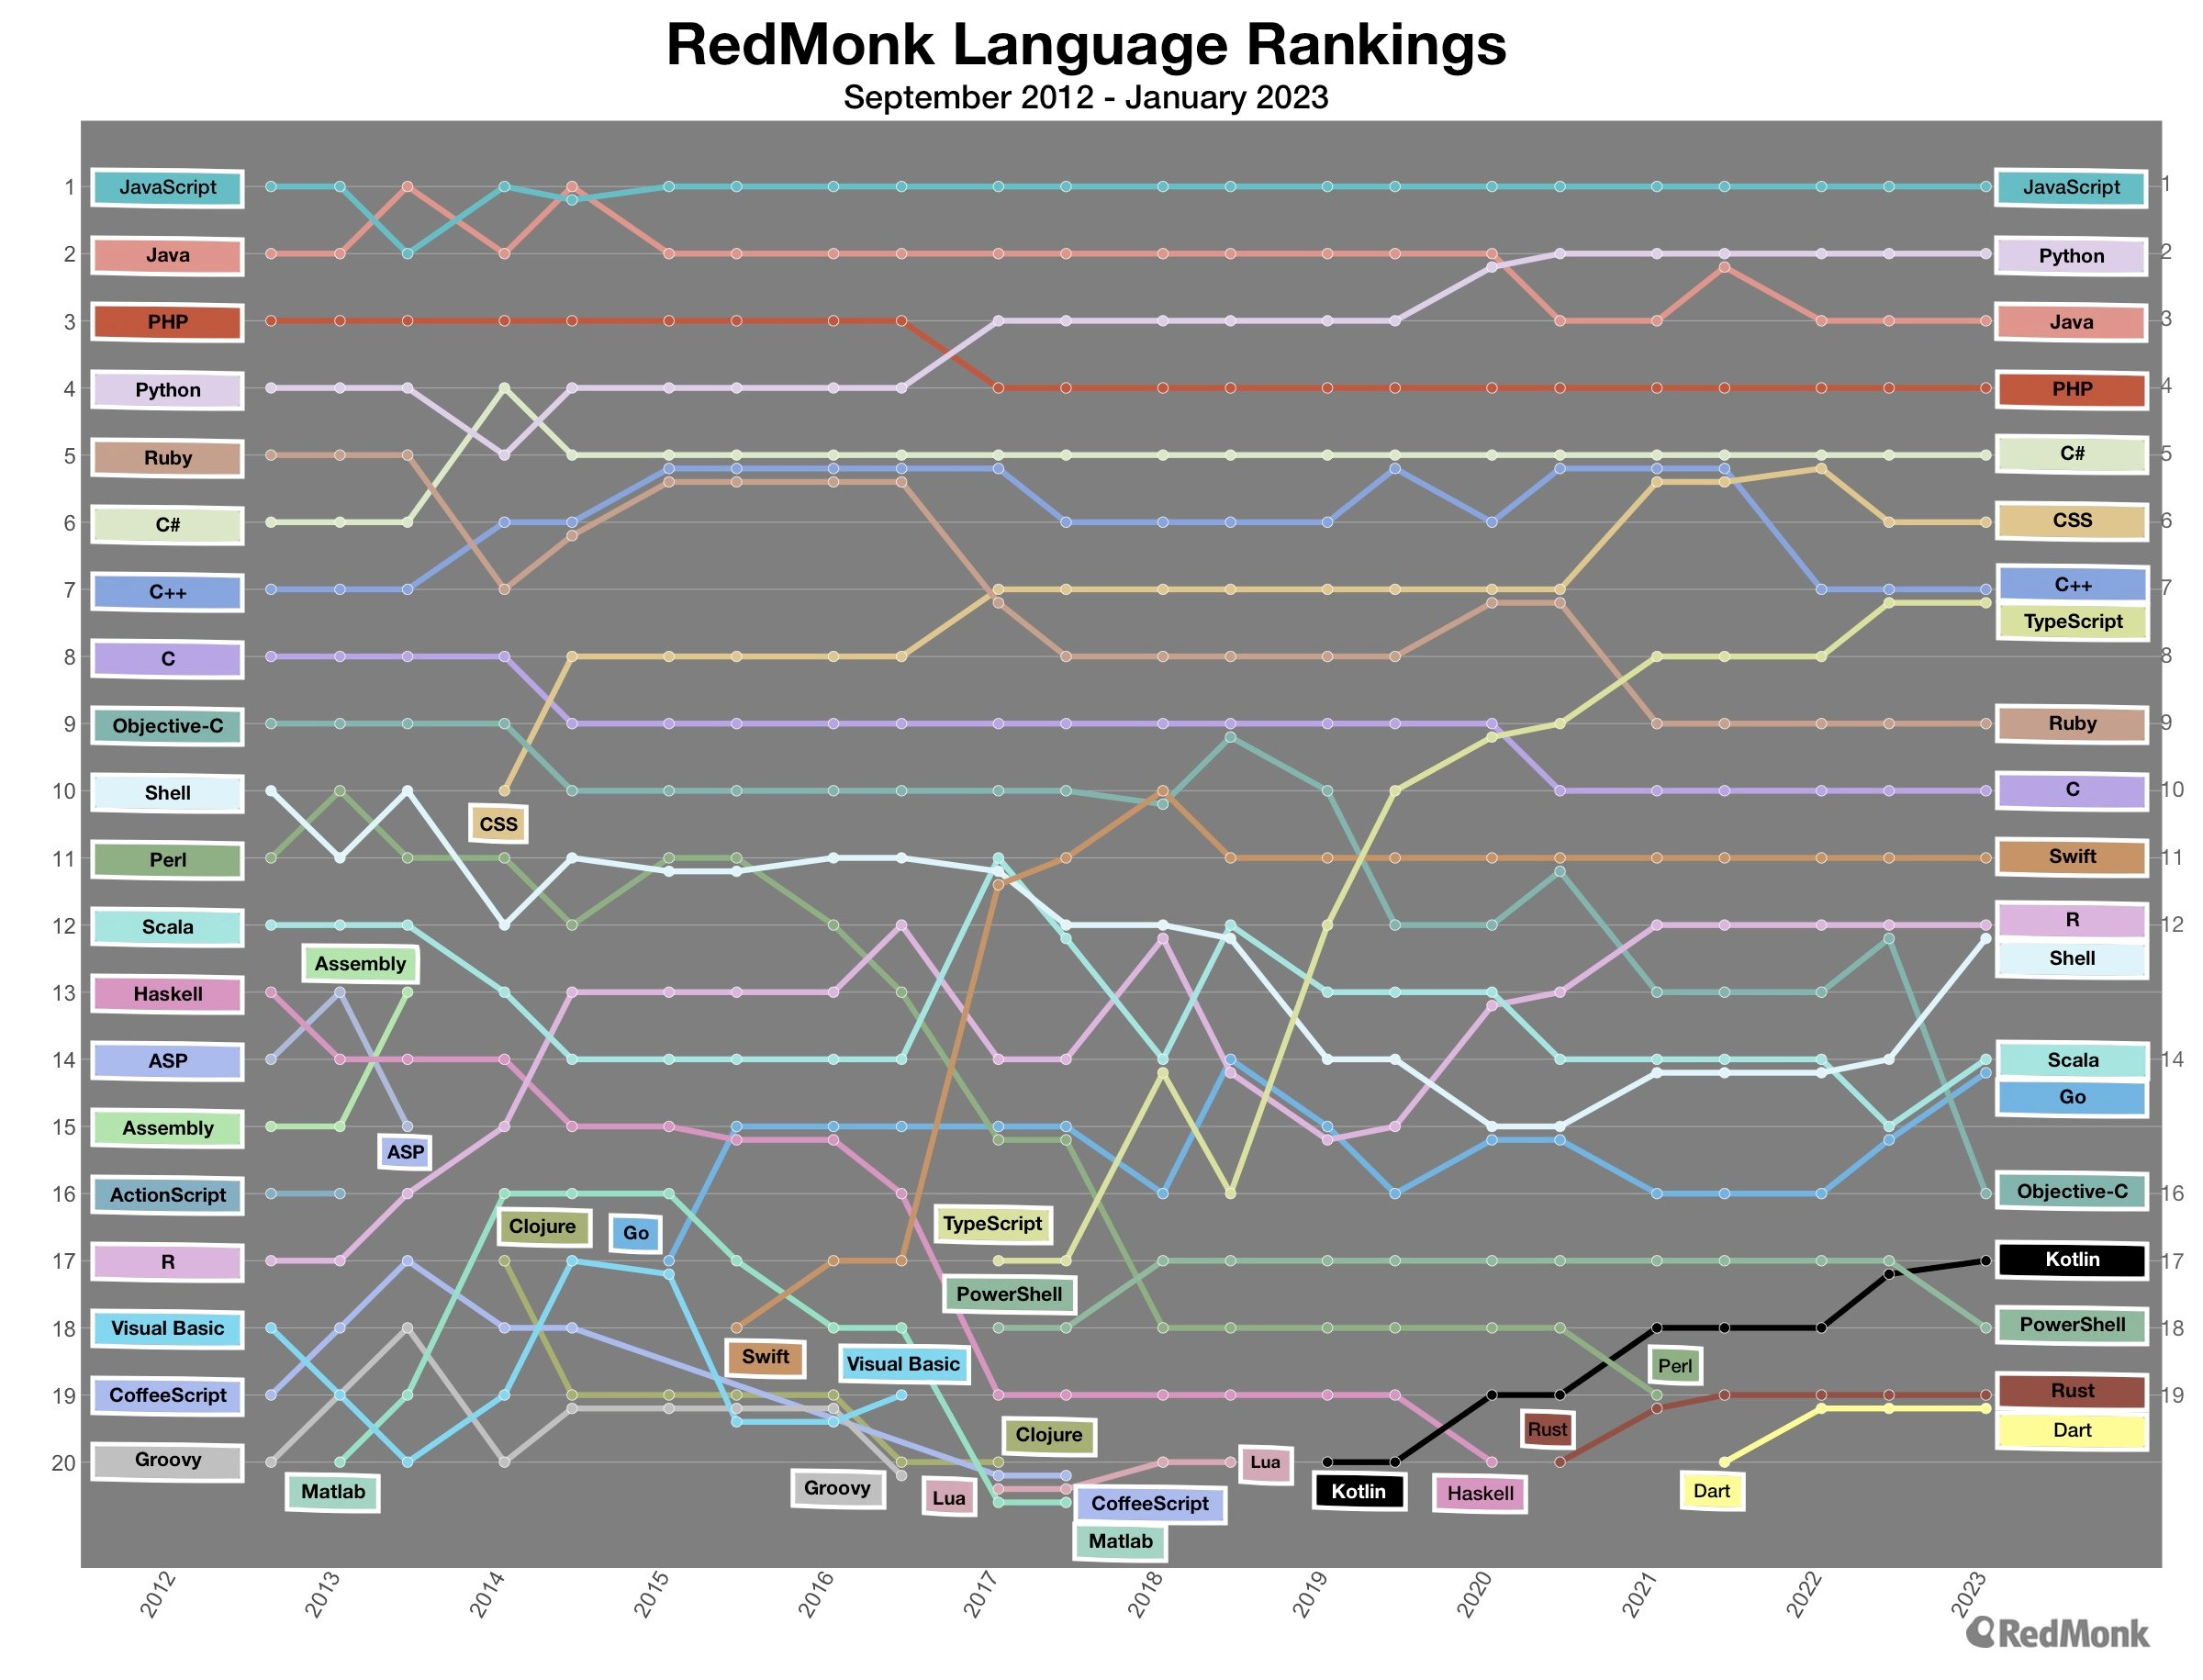
\includegraphics[width=\textwidth]{media/fig1.jpg}
  \caption{Programming Language Popularity Over Time, adapted from
  RedMonk\textquotesingle s 2023 Q1 Programming Language Rankings
  \cite{33}.}
  \label{fig:prog_lang}
\end{figure}

\subsection{Docker for
Containerization}\label{docker-for-containerization}

With Docker, each part of an application, along with its dependencies
and libraries is packaged together in a container. This ensures that the
application runs uniformly regardless of where the container is deployed
\cite{35}.

An alternative to Docker is to manage dependencies manually or use a
virtual environment such as Python\textquotesingle s native venv. While
such options can work, they are not as robust as Docker when it comes to
encapsulating an application and its environment. Specifically, they do
not provide the level of isolation or the ease of deployment that Docker
offers \cite{36}.

\paragraph{Advantages of Using Docker}\label{advantages-of-using-docker}

\begin{itemize}
\item
  \textbf{Isolation}: Containers operate in isolation, ensuring that
  each service is unaware of the other and runs independently.
\item
  \textbf{Version Control for Environments}: Much like source code, the
  Docker environment can be version controlled, enabling easy rollback
  and updates.
\item
  \textbf{Scalability}: Docker makes it easier to create a distributed
  system, facilitating the application\textquotesingle s scaling without
  a hassle.
\item
  \textbf{Easy Deployment}: With Docker, the development environment can
  be precisely replicated in the production system, minimizing
  deployment errors.
\item
  \textbf{Cross-Platform}: Docker containers can run anywhere, on any
  machine that has Docker installed, regardless of the underlying
  operating system.
\end{itemize}

\paragraph{Disadvantages of Using
Docker}\label{disadvantages-of-using-docker}

\begin{itemize}
\item
  \textbf{Learning Curve}: Docker has a learning curve, and initial
  setup can be complex.
\item
  \textbf{Resource Intensive}: Containers may consume more resources
  than native applications when running multiple instances.
\item
  \textbf{Overhead}: For simpler applications, the advantages of Docker
  may not justify the resource overhead and the complexity it
  introduces.
\end{itemize}
